\let\negmedspace\undefined
\let\negthickspace\undefined
\documentclass[journal]{IEEEtran}
\usepackage[a5paper, margin =  10mm, onecolumn]{geometry}
%\usepackage{lmodern} % Ensure lmodern is loaded for pdflatex
\usepackage{tfrupee} % Include tfrupee package

\setlength{\headheight}{1cm} % Set the height of the header box
\setlength{\headsep}{0mm}     % Set the distance between the header box and the top of the text

\usepackage{gvv-book}
\usepackage{gvv}
\usepackage{cite}
\usepackage{amsmath,amssymb,amsfonts,amsthm}
\usepackage{algorithmic}
\usepackage{graphicx}
\usepackage{textcomp}
\usepackage{xcolor}
\usepackage{txfonts}
\usepackage{listings}
\usepackage{enumitem}
\usepackage{mathtools}
\usepackage{gensymb}
\usepackage{comment}
\usepackage[breaklinks =  true]{hyperref}
\usepackage{tkz-euclide} 
\usepackage{listings}
% \usepackage{gvv}                                        
\def\inputGnumericTable{}                                 
\usepackage[latin1]{inputenc}                                
\usepackage{color}                                            
\usepackage{array}                                            
\usepackage{longtable}                                       
\usepackage{calc}                                             
\usepackage{multirow}                                         
\usepackage{hhline}                                           
\usepackage{ifthen}                                           
\usepackage{lscape}
\begin{document}

\bibliographystyle{IEEEtran}
\vspace{1cm}

\title{4.3.23}
\author{EE25BTECH11034 - Kishora Karthik}
% \maketitle
% \newpage
% \bigskip
{\let\newpage\relax\maketitle}

\renewcommand{\thefigure}{\theenumi}
\renewcommand{\thetable}{\theenumi}
%\setlength{\intextsep}{10pt} % Space between text and floats
\textbf{Question:}\\
The line segment joining the points $\vec{A}(3,2)$ and $\vec{B}(5,1)$ is divided at the point $\vec{P}$ in the ratio $1:2$ which lies on $3x - 18y+k=0$. Find the value of k.\\

\textbf{Solution:}\\
Given the points,
\begin{align}
    \vec{A}=\begin{myvec}{3\\2}\end{myvec}\\ 
    \vec{B}=\begin{myvec}{5\\1}\end{myvec}
\end{align}
and the line $L_1$,
\begin{align}
    L_1: \myvec{3 & -18}\vec{x} = -k
\end{align}
\begin{align}
    \implies \vec{n}^{\top}\vec{x}=0
\end{align}
Where,
\begin{align}
     \vec{n}=\myvec{3\\-18}
\end{align}

\bigskip

Let the vector $\vec{P}$ be a point on the line $3x - 18y+k=0$ wihch divides the line segment joining the points $\vec{A}$ and $\vec{B}$.
\\
Section formula for a vector $\vec{P}$ which divides the line formed by vectors $\vec{A}$ and $\vec{B}$ in the ratio $m:1$ is given by
\begin{align}
    \vec{P}=\frac{m\vec{B}+\vec{A}}{m+1}
\end{align}
\begin{align}
	\vec{P}=\myvec{\vec{A} & \vec{B}}\myvec{\frac{1}{m+1}\\\frac{m}{m+1}}
\end{align}
Here, $m=1/2$.
\begin{align}
    \implies \vec{P}=\myvec{\vec{A} & \vec{B}}\myvec{\frac{2}{3}\\\frac{1}{3}}
\end{align}\\
\bigskip

Since $\vec{P}$ lies on line $L_1$,
\begin{align}
    \vec{n}^{\top}\vec{P}=0
\end{align}
\begin{align}
	\implies \myvec{3 &-18}\myvec{\vec{A} & \vec{B}}\myvec{\frac{2}{3}\\\frac{1}{3}}=-k
\end{align}
\begin{align}
    \implies \myvec{3 & -18}\myvec{3 & 5\\2 & 1}\myvec{\frac{2}{3}\\\frac{1}{3}}=-k
\end{align}
\begin{align}
    \implies \myvec{3\cdot 3 + (-18)\cdot 2 & 3\cdot 5 + (-18)\cdot 1}\myvec{\frac{2}{3}\\\frac{1}{3}}=-k
\end{align}
\begin{align}
    \implies \myvec{-27&-3}\myvec{\frac{2}{3}\\\frac{1}{3}}=-k
\end{align}
\begin{align}
    \implies \myvec{(-27)\cdot \frac{2}{3} + (-3)\cdot \frac{1}{3}}=-k
\end{align}
\begin{align}
    \implies k=19
\end{align}
$\therefore$ The value of k is 19 and the equation of the line is $3x - 18y+19=0$.
\centering   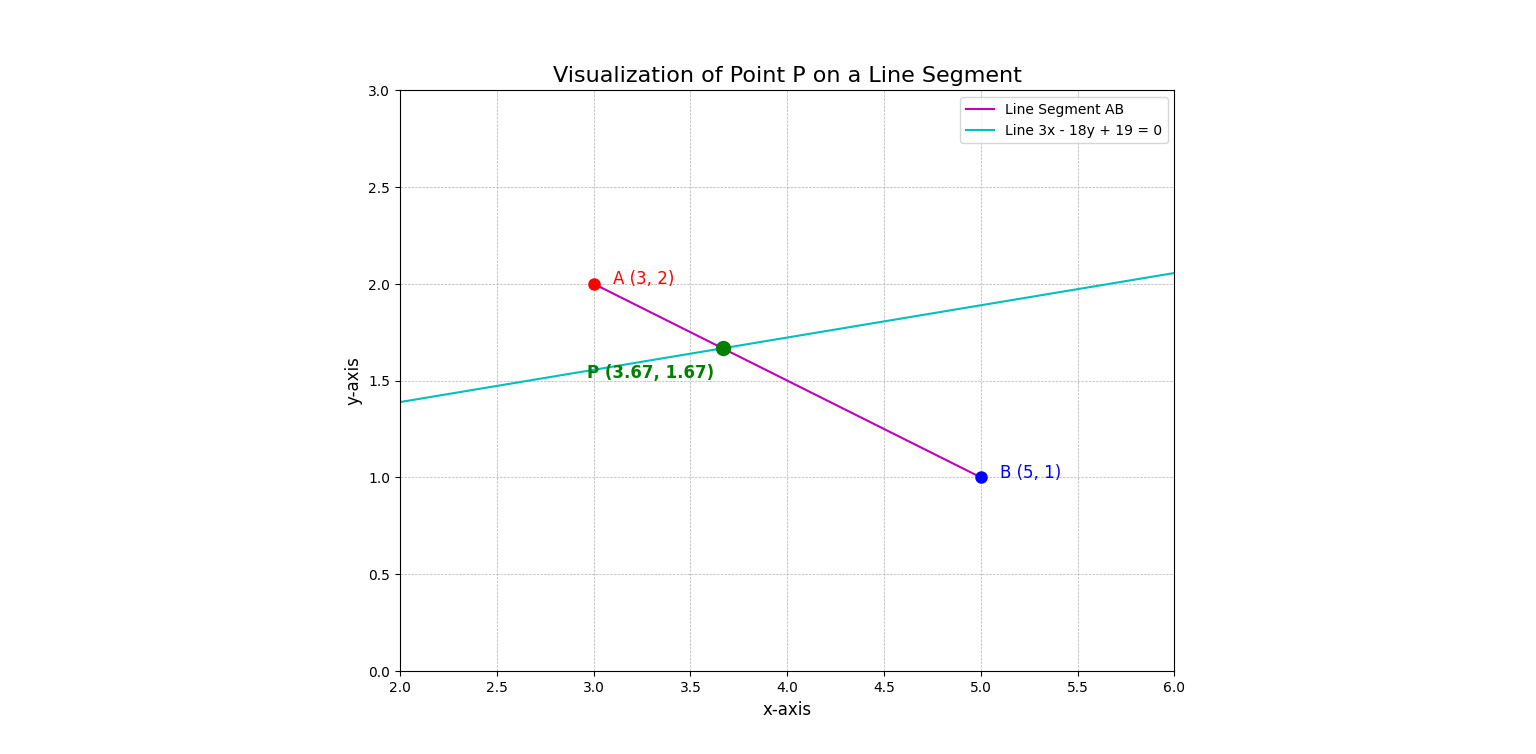
\includegraphics[width=\columnwidth, height=1\textheight, keepaspectratio]{figs/fig1.png} 
\end{document}
